\documentclass[12pt]{article}
\usepackage[letterpaper,margin=.65in,headheight=18pt,headsep=18pt,footskip=25pt]{geometry}
\usepackage[T1]{fontenc}\usepackage{helvet}\renewcommand{\familydefault}{\sfdefault}
\usepackage{tikz,array,fancyhdr}\usetikzlibrary{arrows.meta}
\pagestyle{fancy}\fancyhf{}\renewcommand{\headrulewidth}{0pt}
\fancyhead[L]{\small Week 34 / Hidden turns encore / Grades 2--5}
\fancyfoot[L]{\scriptsize Bellingham Math Circle / Week 34 / W34-BON-v1}\fancyfoot[R]{\scriptsize\thepage}
\setlength{\parindent}{0pt}\setlength{\parskip}{9pt}
\newcommand{\problem}[2]{\par\textbf{Problem #1:} #2\par}
\newcommand{\ring}[5]{\begin{tikzpicture}[x=1cm,y=1cm]
\draw[black!35] (0,0) circle (#2);\foreach \s [count=\i from 0] in {#4}{\coordinate (p) at ({90-360*\i/#1}:#2);\draw[fill=white] (p) circle (#3);\ifnum\pdfstrcmp{\s}{-}=0\else\node[font=\small] at (p){\s};\fi}
\node[anchor=north] at (0,{-#2-#3-.2}){#5};\end{tikzpicture}}
\newcommand{\motion}[2]{\begin{tikzpicture}[x=1cm,y=1cm,>=Stealth]
\draw (0,0) circle (.85);\foreach \i in {0,...,7}{\draw[fill=white] ({90-45*\i}:.85) circle (.08);}
#2\node[anchor=north,align=center,font=\small] at (0,-1.4){#1};\end{tikzpicture}}
\newcommand{\layers}[4]{\begin{tikzpicture}[x=1cm,y=1cm]
\draw[black!35] (0,0) circle (#2);\foreach \i in {0,...,#1}{\ifnum\i<#1\coordinate (p\i) at ({90-360*\i/#1}:#2);\draw[fill=white] (p\i) circle (.25);\fi}
\foreach \i in {#3}{\ifnum\i>-1\fill ([xshift=-2pt]p\i) circle (2pt);\fi}
\foreach \i in {#4}{\ifnum\i>-1\draw[line width=.7pt] ([xshift=1pt,yshift=-2pt]p\i) rectangle +(4pt,4pt);\fi}
\end{tikzpicture}}
\begin{document}
A matching motion puts every counter kind onto the same kind. Kind names stay fixed. Do not count a whole turn. Test flips with a tracing copy while the original stays still.
\problem{1}{Make three A/B patterns on a six-ring: one with exactly one matching flip, one with exactly two, and one with exactly three. Your partner tests every possible flip.}
\begin{center}\begin{tabular}{ccc}
\ring{6}{1.05}{.23}{-,-,-,-,-,-}{1 matching flip}&\ring{6}{1.05}{.23}{-,-,-,-,-,-}{2 matching flips}&\ring{6}{1.05}{.23}{-,-,-,-,-,-}{3 matching flips}
\end{tabular}\end{center}
\begin{center}\ring{6}{3.1}{1.4}{-,-,-,-,-,-}{}\end{center}
\problem{2}{Can a six-ring have exactly four matching flips? Find a pattern or explain why no pattern works.}
\vspace{3cm}
\newpage
\problem{3}{Start with the pattern shown. Change as few counter kinds as possible so that a half-turn matches. Find two different best repairs. Explain why fewer changes cannot work.}
\begin{center}\begin{tabular}{cc}
\ring{8}{1.25}{.28}{A,A,A,B,B,A,B,B}{starting pattern}&\motion{half-turn: 4 spots}{\draw[->,line width=1pt] (90:1.15) arc[start angle=90,end angle=-90,radius=1.15];}
\end{tabular}\end{center}
\begin{center}\ring{8}{3.7}{1.4}{-,-,-,-,-,-,-,-}{}\end{center}
\begin{center}\begin{tabular}{cc}
\ring{8}{1.1}{.24}{-,-,-,-,-,-,-,-}{}&\ring{8}{1.1}{.24}{-,-,-,-,-,-,-,-}{}
\end{tabular}\end{center}
\vspace{1cm}
\newpage
\problem{4}{Start with the same pattern each time. For each motion card, make the fewest changes that let it match. Which motion needs the fewest changes? Explain why your repairs are best.}
\begin{center}\ring{8}{1.5}{.3}{A,A,A,B,B,A,B,B}{starting pattern}\end{center}
\begin{center}\begin{tabular}{ccc}
\motion{flip across this line}{\draw[dashed,line width=1pt] (0,-1.15)--(0,1.15);}&
\motion{turn 1 spot}{\draw[->,line width=1pt] (90:1.15) arc[start angle=90,end angle=45,radius=1.15];}&
\motion{turn 2 spots}{\draw[->,line width=1pt] (90:1.15) arc[start angle=90,end angle=0,radius=1.15];}
\end{tabular}\end{center}
\begin{center}\begin{tabular}{ccc}
\ring{8}{1.35}{.3}{-,-,-,-,-,-,-,-}{flip repair}&\ring{8}{1.35}{.3}{-,-,-,-,-,-,-,-}{1-spot repair}&\ring{8}{1.35}{.3}{-,-,-,-,-,-,-,-}{2-spot repair}
\end{tabular}\end{center}
\vspace{5cm}
\newpage
Each spot may be marked or blank in each layer. Filled dots belong to the first layer; outline squares belong to the second. Keep both marks at an overlap. Only the mark at each spot counts; ignore which way a square faces. Layers cannot be swapped.
\begin{center}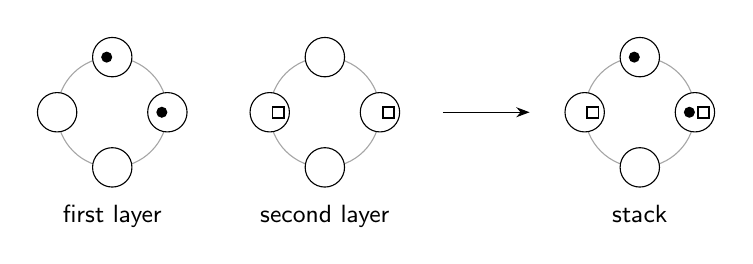
\begin{tikzpicture}[x=1cm,y=1cm,>=Stealth]
\node at (0,0){\layers{4}{.7}{0,1}{-1}};\node[anchor=north,font=\small] at (0,-1.05){first layer};
\node at (2.7,0){\layers{4}{.7}{-1}{1,3}};\node[anchor=north,font=\small] at (2.7,-1.05){second layer};
\node at (6.7,0){\layers{4}{.7}{0,1}{1,3}};\node[anchor=north,font=\small] at (6.7,-1.05){stack};
\draw[->] (4.2,0)--(5.3,0);
\end{tikzpicture}\end{center}
\problem{5}{Make two six-ring layers that each have exactly one matching flip, but whose stack has no matching turn or flip except a whole turn. Find and record both layers and their stack.}
\begin{center}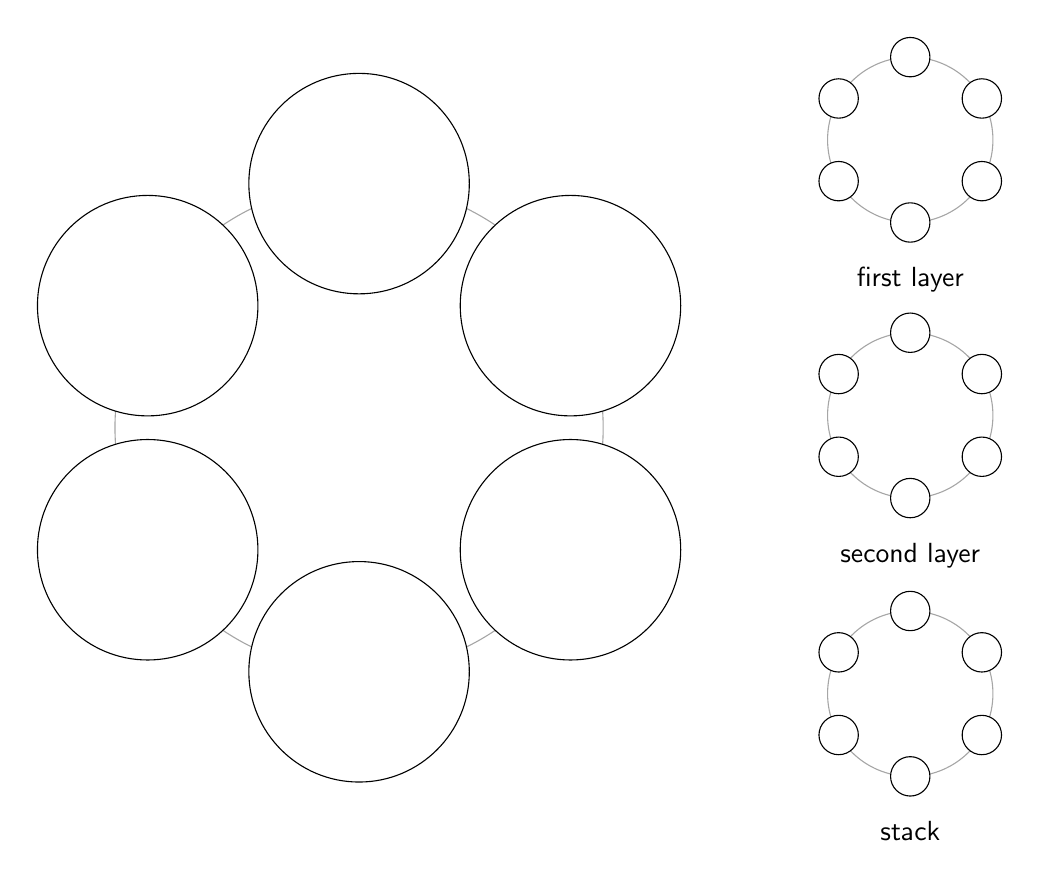
\begin{tikzpicture}[x=1cm,y=1cm]
\node at (0,0){\ring{6}{3.1}{1.4}{-,-,-,-,-,-}{}};
\node at (7,3.5){\ring{6}{1.05}{.25}{-,-,-,-,-,-}{first layer}};
\node at (7,0){\ring{6}{1.05}{.25}{-,-,-,-,-,-}{second layer}};
\node at (7,-3.5){\ring{6}{1.05}{.25}{-,-,-,-,-,-}{stack}};
\end{tikzpicture}\end{center}
\problem{6}{Make two new layers that each match a half-turn. Can their stack fail to match that same half-turn? Explain your answer.}
\begin{center}\begin{tabular}{c@{\hspace{5mm}}c@{\hspace{5mm}}c}
\ring{6}{.95}{.24}{-,-,-,-,-,-}{first layer}&\ring{6}{.95}{.24}{-,-,-,-,-,-}{second layer}&\ring{6}{.95}{.24}{-,-,-,-,-,-}{stack}
\end{tabular}\end{center}
\end{document}
